\subsection{Hidden Markov Models}

HMMs are common statistical models used to describe time series that exhibit state-switching behaviour. An HMM models an observed sequence of length $T$, $\bfY = \{Y_t\}_{t=1}^T$, together with an unobserved (or  ``hidden") sequence $\bfX = \{X_t\}_{t=1}^T$. The hidden sequence $\bfX$ is a Markov chain, and each observation $Y_t$ is a random variable, where $Y_t$ given all other observations $\bfY \setminus \{Y_t\}$ and hidden states $\bfX$ depends only on $X_t$. While the sample space of $\bfX$ is general, we assume $X_t \in \{1,\ldots,N\}$ for some finite $N$. The unconditional distribution of $X_1$ is denoted by the row-vector $\delta \in \bbR^N$, where $\delta^{(i)} = \bbP(X_1 = i)$. Further, the distribution of $X_t$ for $t > 1$ conditioned on $X_{t-1}$ is denoted by an $N$-by-$N$ transition probability matrix $\Gamma_t$, where $\Gamma_t^{(i,j)} = \bbP(X_t = j \mid X_{t-1} = i)$. %Our methods apply to transition probability matrices that depend upon time, but for ease of presentation
For simplicity, we assume that $\Gamma_t$ does not change over time (i.e. $\Gamma_t = \Gamma$ for all $t$) unless stated otherwise. 

%We assume that the distribution of an observation $Y_t$ conditioned on the corresponding hidden state $X_t$ does not depend upon any other observation or hidden state.
%Some variants of HMMs allow $Y_t$ to depend upon both $Y_{t-1}$ and $X_t$. Our methodology can be straightforwardly applied to such HMMs, but for clarity of presentation we assume that $Y_t$ depends only on $X_t$. 
If $X_t=i$, then we denote the conditional density or probability mass function of $Y_t$ as $f^{(i)}(\cdot ; \theta^{(i)})$ or simply $f^{(i)}$, where $\theta^{(i)}$ is a state-dependent parameter describing the emission distribution. The collection of all state-dependent parameters is $\theta = \{\theta^{(i)}\}_{i=1}^N$. Figure \ref{fig:HMM} shows an HMM as a graphical model.

\begin{figure}[h]
    \centering
    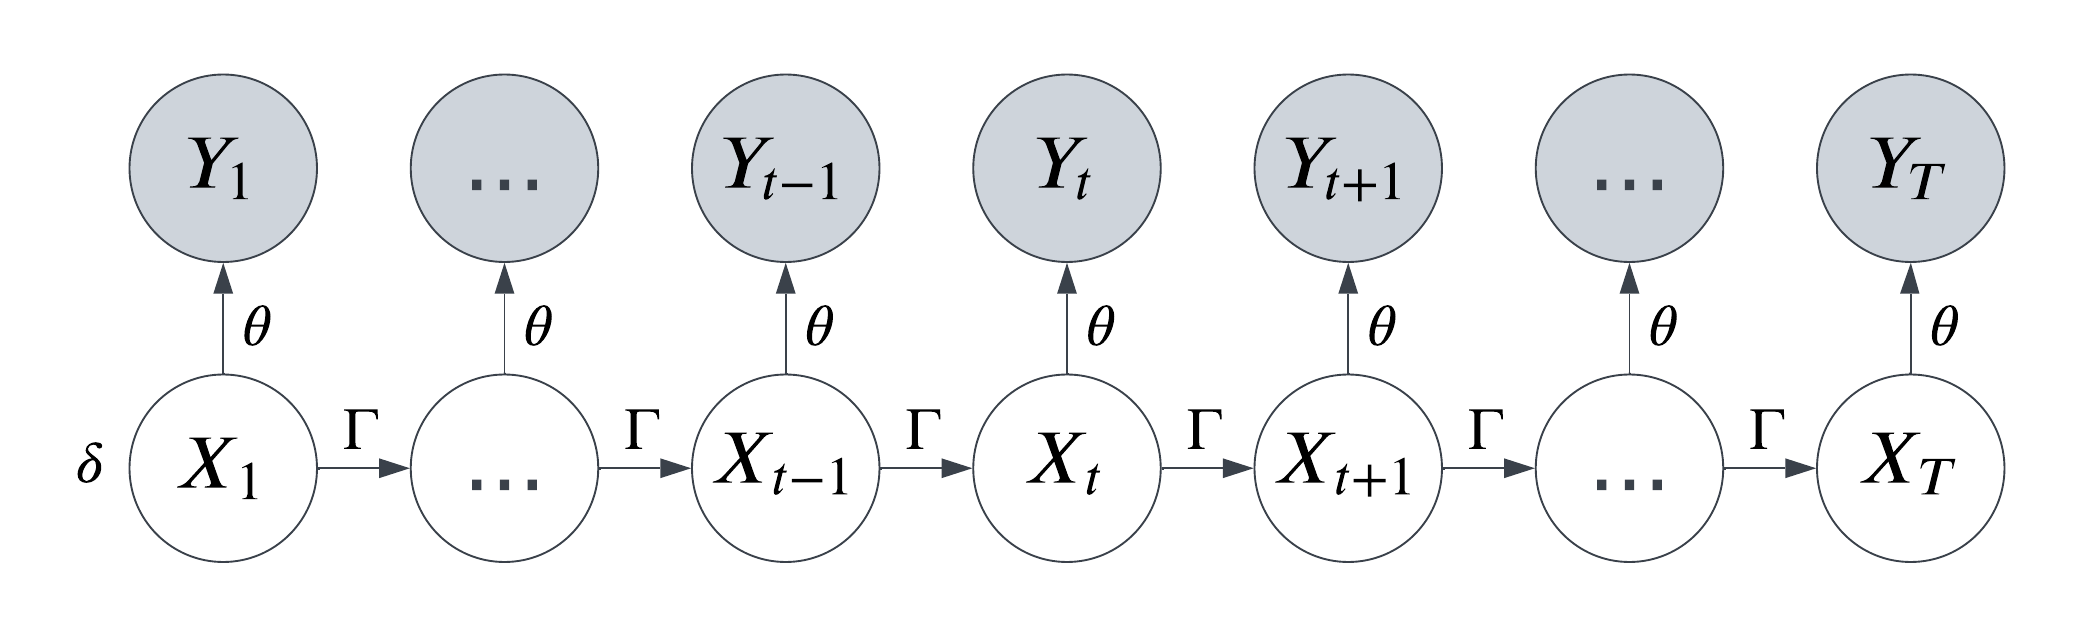
\includegraphics[width=5in]{../plt/HMM.png}
    \caption{Graphical representation of an HMM. $X_t$ corresponds to an unobserved latent state at time $t$ whose distribution is described by a Markov chain. $Y_t$ corresponds to an observation at time $t$, where $Y_t$ given all other observations $\bfY \setminus \{Y_t\}$ and hidden states $\bfX$ depends only on $X_t$.}
    \label{fig:HMM}
\end{figure}

It is convenient to reparameterize the transition probability matrix $\Gamma \in \bbR^{N \times N}$ and initial distribution $\delta \in \bbR^N$ in terms of an auxiliary variable $\eta$ to ensure that all entries are positive and all rows sum to one. One natural option is to use a softmax parameterization: %follow the parameterization of \citet{Barajas:2017}:
%
\begin{equation}
    \Gamma^{(i,j)}(\eta) = \frac{\exp(\eta^{(i,j)})}{\sum_{k=1}^N \exp(\eta^{(i,k)})}, \qquad \delta^{(i)}(\eta) = \frac{\exp(\eta^{(i)})}{\sum_{k=1}^N \exp(\eta^{(k)})}
    \label{eqn:reparam}
\end{equation}
%
where $i,j = 1,\ldots,N$ and $\eta^{(i,i)}$ and $\eta^{(1)}$ are set to zero for identifiability. This formulation simplifies likelihood maximization by removing constraints in the optimization problem. One may also incorporate covariates into $\Gamma$ by setting $\eta_t^{(i,j)}(\beta) = \left(\beta^{(i,j)}\right)^T \bfz_t$, where $\bfz_t$ is a column vector of known covariates at time index $t$ and $\beta^{(i,j)}$ is a column vector of unknown regression coefficients. While $\Gamma$ and $\delta$ are functions of $\eta$, we abuse notation in future sections and treat $\Gamma$ and $\delta$ as variables since the mapping is a bijection.
%
For brevity, we denote $\phi \equiv \{\theta,\eta\}$, $\eta^{(\cdot)} = \{\eta^{(i)}\}_{i=1}^N$, 
$\eta^{(i,\cdot)} = \{\eta^{(i,j)}\}_{j=1}^N$, and $\eta^{(\cdot,\cdot)} = \{\eta^{(i,j)}\}_{i,j=1}^N$. 

The joint likelihood of an HMM given observations $\bfY$ and latent states $\bfX$ is
%
\begin{equation}
    p(\bfX,\bfY;\phi) = \delta^{(X_1)} f^{(X_1)}(Y_1; \theta^{(X_1)}) \prod_{t=2}^T \Gamma^{(X_{t-1},X_t)} f^{(X_t)}(Y_t; \theta^{(X_t)}).
    \label{eqn:like}
\end{equation}
%
Alternatively, the marginal likelihood of the observed data $\bfY$ alone is 
%
\begin{equation}
    p(\bfY;\phi) = \delta P(Y_1;\theta) \prod_{t=2}^T \Gamma P(Y_t;\theta) \mathbf{1}_N.
    \label{eqn:like_marginal}
\end{equation}
%
where $\mathbf{1}_N$ is an $N$-dimensional column vector of ones and $P(y_t;\theta)$ is an $N \times N$ diagonal matrix with the $(i,i)^{th}$ entry $f^{(i)}(y_t; \theta^{(i)})$. For a more complete introduction to HMMs, see \citet{Zucchini:2016}.


\subsection{State Decoding}

One appealing feature of HMMs is that it is simple to determine the probability distribution of the hidden state at time $t$, $X_t$, conditional of the set of observations $Y_t$. Define the probability density of the observations between times $s$ and $t$ as $p(y_{s:t};\phi)$. Likewise, define \textit{forward probabilities} $\alpha^{(i)}_t = p(y_{1:t},X_t = i;\phi)$ (for $i = 1,\ldots,N$ and $t = 1,\ldots,T$) and \textit{backward probabilities} $\beta^{(i)}_t = p(y_{(t+1):T}|X_t = i;\phi)$ (for $i = 1,\ldots,N$ and $t = 1,\ldots,T-1$). By convention, $\beta^{(i)}_T = 1$ for $i = 1,\ldots,N$. Both $\alpha_t$ and $\beta_t$ can be calculated using a recursion. We define the mapping from $\alpha_{t-1}$ and $\phi$ to $\alpha_t$ as $\tilde \alpha_t(\alpha_{t-1},\phi)$, but the value itself is simply $\alpha_t(\phi)$ because $\alpha_t$ is a function of $\phi$ alone. Likewise, we define the mapping from $\beta_{t+1}$ and $\phi$ to $\beta_{t}$ as $\tilde \beta_t(\alpha_{t+1},\phi)$ and the value itself as $\beta_t(\phi)$. 
%
\begin{align}
    \alpha_1^{(i)}(\phi) = \tilde \alpha_1^{(i)}(\phi) \quad &= \quad  \delta^{(i)} ~ f^{(i)} ~ (y_1;\theta^{(i)}), \\
    %
    \alpha_t^{(i)}(\phi) = \tilde \alpha_t^{(i)}(\alpha_{t-1}(\phi),\phi) \quad &= \quad \sum_{j=1}^N ~ \alpha_{t-1}^{(j)}(\phi) ~ \Gamma^{(j,i)} ~ f^{(i)}(y_t;\theta^{(i)}), \quad t = 2,\ldots,T, \label{eqn:alpha} \\
    %
    \beta_T^{(i)}(\phi) = \tilde \beta_T^{(i)}(\phi) \quad &= \quad  1, \\
    %
    \beta_t^{(i)}(\phi) = \tilde \beta_t^{(i)}(\beta_{t+1}(\phi), \phi) \quad &= \quad \sum_{j=1}^N ~ \Gamma^{(i,j)} ~ f^{(j)}(y_{t+1};\theta) ~ \beta^{(j)}_{t+1}(\phi), \quad t = 1,\ldots,T-1. \label{eqn:beta}
\end{align}
%
%It is important to note that $\alpha_t$ and $\beta_t$ are functions of $\phi$ alone. We nonetheless abuse notation and write $\alpha_t$ and $\beta_t$ as functions of $\alpha_{t-1}$ and $\beta_{t+1}$ as well to illustrate the recursion. In addition, it takes $\calO(N^2)$ time to calculate $\alpha_{t}$ and $\beta_{t}$ if $\alpha_{t-1}$, $\beta_{t+1}$, and $\phi$ are known. However, it takes $\calO(TN^2)$ time to calculate $\alpha_{t}$ and $\beta_{t}$ if only $\phi$ is known, as the recursions starting from $\alpha_1$ and $\beta_T$ must be performed.
%
Note that it takes $\calO(N^2)$ time to evaluate $\tilde \alpha_t$ and $\tilde \beta_t$, but $\calO(TN^2)$ time to evaluate $\alpha_t(\phi)$ and $\beta_t(\phi)$. In future sections we abuse notation and write $\alpha_t(\phi)$ and $\beta_t(\phi)$ as $\alpha_t$ and $\beta_t$ for brevity. 

We denote the probability that $X_t = i$ given all observations $\bfY$ and parameters $\phi$ as $\gamma_t^{(i)}(\phi)$ for $t = 1,\ldots,T$ and $i = 1,\ldots,N$. Further, we denote the probability that $X_{t-1} = i$ and $X_t = j$ given all observations $\bfY$ and parameters $\phi$ as $\xi_t^{(i,j)}(\phi)$ for $t = 2,\ldots,T$ and $i,j = 1,\ldots,N$. Namely,
%
\begin{gather}
    \gamma_t^{(i)}(\phi) = \bbP(X_t = i \mid \bfY ~;~ \phi), \\ \xi_t^{(i,j)}(\phi) = \bbP(X_{t-1} = i, X_t = j \mid \bfY ~;~ \phi).
\end{gather}
%
Both $\gamma_t$ and $\xi_t$ can be calculated from $\alpha_{t-1}$, $\alpha_t$, $\beta_t$, and $\phi$:
%
\begin{align}
    \gamma_t^{(i)}(\phi) = \tilde \gamma_{t}^{(i)}(\alpha_t,\beta_t) \quad &= \quad   \frac{\alpha_{t}^{(i)} ~ \beta_{t}^{(i)}}{\sum_{i'} \alpha_{t}^{(i')} ~ \beta_{t}^{(i')}}, \label{eqn:gamma} \\
    %
    \xi_{t}^{(i,j)}(\phi) = \tilde \xi_{t}^{(i,j)}(\alpha_{t-1},\beta_{t},\phi) \quad &= \quad \frac{\alpha_{t-1}^{(i)} ~ \Gamma^{(i,j)} ~ f^{(j)}(y_{t} ~ ; ~\theta) ~ \beta_{t}^{(j)}}{\sum_{i',j'} ~ \alpha_{t-1}^{(i')} ~ \Gamma^{(i',j')} ~ f^{(j')}(y_{t} ~ ; ~\theta) ~ \beta_{t}^{(j')}} \label{eqn:xi}.
\end{align}
%
It takes $\calO(N^2)$ time to evaluate $\tilde \gamma_{t}(\alpha_t,\beta_t)$ and $\tilde \xi_{t}^{(i,j)}(\alpha_{t-1},\beta_{t},\phi)$, but $\calO(TN^2)$ time to evaluate $\gamma_t(\phi)$ and $\xi_t(\phi)$. In future sections we abuse notation and write $\gamma_t(\phi)$ and $\xi_t(\phi)$ as $\gamma_t$ and $\xi_t$ for brevity. 

\subsection{The Baum-Welch Algorithm}

The Baum-Welch algorithm is a specific instance of the EM algorithm used to estimate the parameters of the HMM. Suppose a sequence of observations $\bfY$ is observed as output of an latent-variable model with unknown latent states $\bfX$ and unknown parameters $\phi$. At iteration $k$ of the EM algorithm, denote the current parameter estimates as $\phi_{k}$. One iteration of the EM algorithm consists of and expectation (or E) step, followed by a maximization (or M) step. For the E step, the function $Q(\phi \mid \phi_{k})$ is defined as the expected value of the joint log-likelihood $\log p(\bfY,\bfX; \phi)$ when $\bfX$ is a random variable with density $p(\bfX | \bfY ; \phi_{k})$. For the M step, the next parameter estimate $\phi^{k+1}$ is found by maximizing $Q(\phi \mid \phi_{k})$ with respect to the parameters $\phi$:
%
\begin{gather}
    Q(\phi \mid \phi_{k}) \equiv \bbE_{\phi_{k}}\left[\log p(\bfY,\bfX;\phi) \mid \bfY \right] \label{eqn:Q} \\
    %
    %Q^*(\phi_{k}) \equiv \max_{\phi}Q(\phi \mid \phi_{k})\\
    %
    \phi_{k+1} = \argmax_{\phi} Q(\phi \mid \phi_{k}). \label{eqn:BW_update}
\end{gather}
%
When the EM algorithm is applied to HMMs, it is called the \textit{Baum-Welch} algorithm. We combine Equation (\ref{eqn:Q}) with Equation (\ref{eqn:like}) to write $Q$ into separate terms: %separate the expected value into three convenient terms:
\begin{align}
    Q(\phi \mid \phi_{k}) &\equiv \bbE_{\phi_{k}}\left[\log p(\bfY,\bfX;\phi) \mid \bfY \right] \\
    %
    &= \bbE_{\phi_{k}} \left[\sum_{t=1}^T \log f^{(X_t)}(y_t;\theta^{(X_t)}) + \log \delta^{(X_1)} + \sum_{t=2}^{T} \log \Gamma^{(X_{t-1},X_{t})} \mid \bfY \right] \\
    %
    &= \sum_{t = 1}^T \bbE_{\phi_{k}} \left[ \log f^{(X_t)}(y_t;\theta^{(X_t)}) \mid \bfY \right]  \\
    & \qquad + \bbE_{\phi_{k}} \Big[\log \delta_{X_1} \mid \bfY \Big] + \sum_{t=2}^{T} \bbE_{\phi_{k}} \left[ \log \Gamma^{(X_{t-1},X_{t})} \mid \bfY \right] \\
    %
    &= \sum_{t = 1}^T \sum_{i=1}^N \gamma^{(i)}_t(\phi_{k}) \log f^{(i)}(y_t;\theta^{(i)}) \\
    & \qquad + \sum_{i=1}^N \gamma^{(i)}_1(\phi_{k}) \log \delta^{(i)} + \sum_{t=2}^{T} \sum_{i=1}^N \sum_{j=1}^N \xi_t^{(i,j)}(\phi_{k}) \log \Gamma^{(i,j)}
\end{align}
%The first term and last two terms on the right-hand side of the equation above only depend upon $\theta$ and $\eta$, respectively. The maximization problem in Equation (\ref{eqn:BW_update}) can thus be divided into two separate sub-problems as follows. Note that we define the objective functions $F$ and $G$ below so that the M-step of the EM algorithm is a minimization problem consistent with existing optimization literature.
%
%\begin{gather}
%    F_t^{(k)}(\theta) \equiv F_t(\theta, \phi_{k}) \equiv - \sum_{i=1}^N \gamma^{(i)}_t(\phi_{k}) \log f^{(i)}(y_t;\theta^{(i)}), \\
    %
%    F^{(k)}(\theta) \equiv F(\theta, \phi_{k}) \equiv \frac{1}{T} \sum_{t=1}^T F^{(k)}_t(\theta), \label{eqn:F} \\
    %
%    \theta_{k+1} = \argmin_{\theta} F^{(k)}(\theta), \label{eqn:EM_update_theta} \\ \nonumber \\
    %
    %
%    G_1^{(k)}(\eta) \equiv G_1(\eta, \phi_{k}) \equiv - \sum_{i=1}^N \gamma^{(i)}_1(\phi_{k})\log \delta^{(i)}(\eta) \\
    %
%    G_t^{(k)}(\eta) \equiv G_t(\eta, \phi_{k}) \equiv - \sum_{i=1}^N \sum_{j=1}^N \xi^{(i,j)}_t(\phi_{k}) \log \Gamma^{(i,j)}(\eta), \quad t \geq 2 \\
    %
%    G^{(k)}(\eta) \equiv G(\eta, \phi_{k}) = \frac{1}{T} \sum_{t=1}^{T} G_t(\eta, \phi_{k}), \label{eqn:G}\\
    %
%    \eta_{k+1} = \argmin_{\eta} G(\eta,\phi_{k}). \label{eqn:EM_update_eta}
%\end{gather}
%In addition, note that 
%\begin{equation}
%   Q(\phi \mid \phi_{k}) = -T ~ \left[F(\theta, \phi_{k}) + G(\eta, \phi_{k})\right].
%\end{equation}
%
More detailed pseudo code for the E and the M step are given in Algorithms (\ref{alg:E}) and (\ref{alg:EM}) below.

\begin{algorithm}
\caption{\texttt{E}($\phi_k$)}\label{alg:E}
\begin{algorithmic}[1]
\Require Parameter value $\phi_k$.
%
\State $\alpha_1 \gets \tilde \alpha_1(\phi_k)$
\State $\beta_T \gets \tilde \beta_T(\phi_k)$
\For{$t = 2,\ldots,T$}
    \State $\alpha_t \gets \tilde \alpha_t(\alpha_{t-1},\phi_k)$
    \State $\beta_{T+1-t} \gets \tilde \beta_t(\beta_{T+2-t},\phi_k)$
\EndFor

\State \Return $\{\alpha_t,\beta_t\}_{t=1}^T$
\end{algorithmic}
\end{algorithm}

\begin{algorithm}
\caption{\texttt{Baum-Welch}$(\phi_0,K)$}\label{alg:EM}
\begin{algorithmic}[1]
\Require Initial parameter values $\phi_0$, number of iterations $K$
\For{$k = 0,\ldots,K-1$}
    \State $\{\alpha_t,\beta_t\}_{t=1}^T \gets \texttt{E}(\phi_{k})$ \Comment{E step} 
    \State $\gamma_1 \gets \tilde \gamma_1(\alpha_{1},\beta_{1})$
    \For{$t = 2,\ldots,T$}
        \State $\gamma_t \gets \tilde \gamma_t(\alpha_{t},\beta_{t})$
        \State $\xi_t \gets \tilde \xi_t(\alpha_{t-1},\beta_{t},\phi_{k})$
    \EndFor
    \State \Comment{M step} $$\phi_{k+1} \gets \argmax_{\{\theta,\eta\}} \sum_{t = 1}^T \sum_{i=1}^N \gamma^{(i)}_t \log f^{(i)}(y_t;\theta^{(i)}) + \sum_{i=1}^N \gamma^{(i)}_1 \log \delta^{(i)}(\eta) + \sum_{t=2}^{T} \sum_{i=1}^N \sum_{j=1}^N \xi_t^{(i,j)} \log \Gamma^{(i,j)}(\eta)$$
\EndFor
\State \Return $\phi_K$
\end{algorithmic}
\end{algorithm}

In many simple scenarios the maximization problem above has a closed-form solution. For example, if $\Gamma$ does not depend upon any covariates and $f^{(i)}(y_t;\theta^{(i)})$ is a normal or Poisson probability density function with respect to $y_t$, then the solution of Equation (\ref{eqn:BW_update}) is given in Section 4.2 of \citet{Zucchini:2016}. However, in many other situations, the maximization problem above is not straightforward and requires numerical maximization techniques. %For example, finding closed-form solutions to the M-step for the HHMM defined in section \ref{subsec:HHMM} is not straightforward. 
We therefore review different methods for numerical maximization via stochastic optimization. %We describe several such scenarios in the subsequent section. 

\subsection{Stochastic Optimization}
\label{subsec:stoch_optim}

Stochastic optimization techniques can solve minimization problems in which the objective function can be written as the sum of independent terms \citep{Robbins:1951}. In much of the stochastic optimization literature, this optimization problem takes the form of a minimization over an average:
%
\begin{equation}
    \phi^* = \argmin_{\phi} F(\phi), \qquad F(\phi) = \frac{1}{T}\sum_{t = 1}^T F_t(\phi).
    \label{eqn:stoch_opt}
\end{equation}
%

Within the M step of the $k^{th}$ iteration of the EM algorithm, standard gradient descent at a given step $m$ with step size $\lambda$ updates $\phi_{k,m}$ as follows:
%
\begin{equation}
    \phi_{k,m} = \phi_{k,m-1} - \lambda \nabla F^{(k)}(\phi_{k,m-1}) =  \phi_{k,m-1} - \frac{\lambda}{T} \sum_{t=1}^T \nabla F^{(k)}_t(\phi_{k,m-1}).
\end{equation}
%
However, this update requires evaluating a gradient for all $t = 1,\ldots,T$, which can be prohibitively expensive if $T$ is large. Alternatively, \citet{Robbins:1951} introduce stochastic gradient descent (or SGD), which updates $\phi_k$ using an unbiased estimate of the full gradient:
%
\begin{equation}
    \phi_{k,m} = \phi_{k,m-1} - \lambda \nabla F^{(k)}_{t_{k,m}}(\phi_{k,m-1})
\end{equation}
%
for some $t_{k,m} \in \{1,\ldots,T\}$ selected uniformly at random at step $m$ of M-step $k$. Stochastic gradient descent reduces the amount of time between updates by using an unbiased estimate of the gradient to update $\phi_{k,m-1}$. However, the gradient estimates themselves can have high variance, so stochastic gradient descent requires that the step-size $\lambda$ decays over time to ensure convergence. In addition, SGD has slower convergence rates compared to full gradient descent \citep{Schmidt:2017}.

Variance-reduced stochastic optimization techniques such as stochastic average gradient descent (SAG) \citep{Schmidt:2017}, stochastic variance reduced gradient descent (SVRG) \citep{Johnson:2013}, and SAGA \citep{Defazio:2014} enjoy the speed of stochastic gradient descent as well as the convergence rates of full gradient descent. These algorithms involve a table of gradient estimates $\widehat \nabla F^{(k)}_t$ whose average approximates the full gradient $\nabla F^{(k)}(\phi_{k,m-1})$. The gradient estimates are updated at various stages in the optimization algorithm and are used to reduce the variance of gradient estimates. 
%In particular, SAG uses the update rule:
%
%\begin{equation}
%    \phi_{m+1} \gets \phi_{m} - \lambda \left[\frac{\nabla F^{(k)}_{t_m}(\phi_{m}) - \widehat \nabla F^{(k)}_{t_m}}{T} + \frac{1}{T} \sum_{t=1}^T \widehat \nabla F^{(k)}_{t} \right], \label{eqn:SAG_update}
%\end{equation}
%
%which is simply the table average with entry $t_m$ updated at step $m$. This update rule is intuitive, but it represents a biased estimate of the gradient $\nabla P(\phi_m)$. This can slow down convergence and makes theoretical analysis of SAG difficult. 
For example, SVRG and SAGA update $\phi$ using an unbiased estimate of the gradient:
%
\begin{equation}
    \phi_{k,m} = \phi_{k,m-1} - \lambda \left[\nabla F^{(k)}_{t_{k,m}}(\phi_{k,m-1}) - \widehat \nabla F^{(k)}_{t_{k,m}} + \widehat \nabla F^{(k)} \right],
    \label{eqn:SAGA_update}
\end{equation}
%
where:
%
\begin{equation}
    \widehat \nabla F^{(k)} = \frac{1}{T} \sum_{t=1}^T \widehat \nabla F^{(k)}_{t}.
    \label{eqn:tbl_avg}
\end{equation}
%Taking the expected value of the gradient estimate from (\ref{eqn:SAGA_update}) shows that it is unbiased:
%
%\begin{align}
%    \bbE\left[\nabla F^{(k)}_{t_m}(\phi_{m}) - \widehat \nabla F^{(k)}_{t_m} + \frac{1}{T} \sum_{t=1}^T \widehat \nabla F^{(k)}_{t} \right] &= \frac{1}{T} \sum_{t=1}^T \nabla F^{(k)}_{t}(\phi_{m}) - \frac{1}{T} \sum_{t=1}^T \widehat \nabla F^{(k)}_{t} + \frac{1}{T} \sum_{t=1}^T \widehat \nabla F^{(k)}_{t} \\
    %
%    &= \frac{1}{T} \sum_{t=1}^T \nabla F^{(k)}_{t_m}(\phi_{m}) = \nabla F^{(k)}(\phi_{m}).
%\end{align}
%
After updating the parameters at step $m$ of iteration $k$, SAGA simply updates the table average and the table of gradients at position $t_{k,m}$: 
%
\begin{gather}
    \widehat \nabla F^{(k)} \gets \widehat \nabla F^{(k)} + \nabla F^{(k)}_{t_{k,m}}(\phi_{k,m}) - \widehat \nabla F^{(k)}_{t_{k,m}}, \\
    %
    \widehat \nabla F^{(k)}_{t_{k,m}} \gets \nabla F^{(k)}_{t_{k,m}}(\phi_{k,m}).
\end{gather}
%
%After updating the table at position $t_m$ with the SAG/SAGA update rule, the table average $\frac{1}{T} \sum_{t=1}^T \widehat \nabla F^{(k)}_{t}$ must be updated using the previous estimate of $\widehat \nabla F^{(k)}_{t}$. 

Traditionally, SAGA is more memory intensive than SVRG because the gradient at every index must be stored. However, the Baum-Welch algorithm involves storing weights for each time index $t$ to define the $Q-$ function, so storing each gradient for SAGA is not any more memory intensive than the Baum-Welch algorithm itself. Alternatively, SVRG is more computationally intensive than SAGA partially because it requires the table average $\widehat \nabla F$ to be occasionally refreshed, which involves a full pass of the data set. However, the E-step of the Baum-Welch algorithm involves a full pass of the data set, using SVRG is not any more computationally expensive than the Baum-Welch algorithm itself. Therefore, using either algorithm in the M-step of the Baum-Welch algorithm adds minimal computational and memory complexity.

%This trade-off should be considered by practitioners when deciding between the two algorithms. 

Algorithm (\ref{alg:SO}) outlines one iteration of SVRG or SAGA in pseudocode. \texttt{VRSO} stands for variance-reduced stochastic optimization.

\begin{algorithm}
\caption{\texttt{VRSO}$(F^{(k)},\phi_0,\lambda,A,M)$}\label{alg:SO}
\begin{algorithmic}[1]
\Require loss function $F^{(k)} = \frac{1}{T}\sum_{t=1}^T F^{(k)}_t$, initial parameter $\phi_0$, step size $\lambda$, algorithm $A \in \{\text{SVRG, SAGA}\}$, and number of iterations $M$.
%
\vspace{5pt}
\For{$t = 1,\ldots,T$}
\State $\gamma_t \gets \tilde \gamma_t(\alpha_t,\beta_t)$
\State $\xi_t \gets \tilde \xi_t(\alpha_{t-1},\beta_{t},\phi_0)$
\State $\widehat \nabla F_t \leftarrow \nabla F_t (\phi_0 \mid \gamma_t,\xi_t)$
\Comment{initialize gradients}
\EndFor
\State $\widehat \nabla F \gets \frac{1}{T} \sum_{t=1}^T \widehat \nabla F_{t}$
\Comment{initialize table average}
%
\For{$m = 1,\ldots,M$}:
    %
    \State Pick $t_{m} \in \{1,\ldots,T\}$ uniformly at random.
    %
    \State \Comment{update parameters}
    \begin{gather}
        \phi_{m} = \phi_{m-1} - \lambda \left[\nabla F_{t_m}(\phi_{m-1} \mid \gamma_{t_m}, \xi_{t_m}) - \widehat \nabla F_{t_{m}} + \widehat \nabla F \right]
        \label{eqn:SAGA_update0}
    \end{gather}
    %
    \If{$A$ = SAGA}:
    \Comment{update table average and table at index $t_{m}$}
        \begin{gather}
            \widehat \nabla F \gets \widehat \nabla F + \frac{1}{T} \left( \nabla F_{t_m}(\phi_{m-1} \mid \gamma_{t_m}, \xi_{t_m}) - \widehat \nabla F_{t_{m}}\right), \\
            \widehat \nabla F_{t_{m}} \gets \nabla F_{t_m}(\phi_{m-1} \mid \gamma_{t_m}, \xi_{t_m}).
        \end{gather}
    \EndIf
\EndFor
\State \Return $\phi_M$
\end{algorithmic}
\end{algorithm}


%Whether or not Equations (\ref{eqn:EM_update_theta}) and (\ref{eqn:EM_update_eta}) have closed-form solutions, even defining $F^{(k)}$ and $G^{(k)}$ to initialize the optimization problem (the E-step) has a time cost of $\calO(T)$, which can be expensive for large $T$. 


%%%%%%%%%%%%